\documentclass{scrartcl}
\usepackage{fontspec} %connects to native fonts
\usepackage{amsmath}
\usepackage{mathtools}
\usepackage{cleveref}
\usepackage{pgfplots}
\usepackage{graphicx}
\usepackage{wrapfig}
\usepackage{fancyref}
\usepackage{amssymb}
\usepackage{subfig}
\usepackage{float}
\usepackage[justification=RaggedRight, singlelinecheck=false, font={footnotesize}]{caption}
\usepackage[portuguese]{babel}
\usepackage[title,titletoc,toc]{appendix}


\usepackage{lipsum}
\usepackage{blindtext}
\addtokomafont{sectioning}{\rmfamily}

\begin{document}
\pagenumbering{arabic}
\bibliographystyle{plain}
\title{
	\textnormal{
	\LARGE Universidade de Lisboa - Instituto Superior Técnico\\
	\Large Licenciatura em Engenharia Informática e de Computadores\\
	\Large Análise e Síntese de Algoritmos
\\}
	\LARGE1º Projeto
	\vspace{-1ex}
	}
\author{Gonçalo Marques,
	\texttt{84719}
	\and
	Manuel Sousa,
	\texttt{84740}
}
\date{	\vspace{-1ex}
		\vspace{-4ex}
	}
\maketitle
%		{\large Universidade de Lisboa}\\[0.4cm]
%		{\large Instituto Superior Técnico}\\[0.4cm]
%		{\large Licenciatura em Engenharia Informática e de Computadores}\\[1.5cm]
\section*{Introdução}
Com este projeto pretendemos expor um algoritmo eficiênte, explicar a sua implementação e fazer uma análise teórica e experimental da complexidade temporal e espacial do mesmo.

\section*{Descrição do problema}
O problema descrito pedia para, dentro de uma rede social onde a informação pode ser partilhada entre todas as pessoas da rede, encontrar pessoas que são fundamentais para a transmissão de informação. Isto é, pessoas que ao serem removidas da rede social tornam impossível a transmissão de informação entre todos os membros da rede.

Ora este problema pode ser descrito como um problema num grafo não direcionado, em que:
\begin{itemize}
\setlength\itemsep{-0.5ex}
\item cada pessoa é um nó da rede
\item uma ligação entre pessoas corresponde a uma aresta
\item o grafo é conexo. ("existe sempre uma forma de partilha de informação entre qualquer par de pessoas")
\end{itemize}

Assim, o problema descrito é equivalente ao de encontrar num grafo conexo $G(V,E)$ (com $N = \#V$ e $L = \#E$) nós que se forem removidos tornam o grafo desconexo, ou seja, de encontrar nós de corte (articulation points).

\section*{Algoritmo utilizado}
Tendo solução do problema sido estudada nas aulas, foi utilizado o algoritmo estudado - o algoritmo de Tarjan para encontrar nós de corte - descrito como \textit{biconnected components algorithm} em \cite{Hopcroft:EAGM}. A descrição do algoritmo será baseada na noção de tempo de descoberta, mas não será utilizada a pilha auxiliar, uma vez que não é necessário encontrar componentes fortemente conexos.

\section*{Estruturas utilizadas:}
\begin{itemize}
\setlength\itemsep{-0.5ex}
\item \textbf{G[$u$][i]} - O grafo $G$ foi representado como uma lista de adjacências (foi utilizado um std::vector (array dinâmica) em vez de std::list (lista duplamente ligada), pelo facto de a implementação do std::vector ser bastante mais eficiente que a de std::list \cite{ISOC++:2003}).
\item \textbf{disco[$u$]} - tempo de descoberta do nó $u$
\item \textbf{low[$u$]} - tempo do mínimo valor de descoberta alcançável sem usar a aresta que retorna ao pai na àrvore DFS a partir do nó $u$
\item \textbf{parent[$u$]} - nó pai do nó $u$ na àrvore DFS
\item \textbf{AP[$u$]} - o nó $u$ é Articulation Point?
\end{itemize}
Todas estas estruturas foram implementadas com o std::vector de C++ que tem tempo de inserção no fim $O(1+)$ e de acesso $O(1)$. Com tempo de inserção $O(1+)$ (constante amortizado), queremos dizer que para inserir $N$ elementos a complexidade de pior caso é $O(N)$, apesar da complexidade de pior caso de inserção de 1 elemento não ser $O(1)$ (de facto é também $O(N)$). \cite{ISOC++:2003}


\section*{Explicação do algoritmo}
 Para o caso de um grafo conexo não-direcionado com pelo menos 2 nós, é executada uma pesquisa em profundidade ao longo dos nós, a partir do nó 1. Para cada nó visitado na DFS é guardada informação relativa ao tempo de descoberta (vetor disco) e ao valor do tempo de descoberta do nó com menor tempo de descoberta acessível a partir do nó atual utilizando apenas arestas ainda não visitadas (vetor low). Se após uma chamada recursiva retornar, o valor de low do filho visitado for superior ao do pai então o pai é um nó de corte.\\
Após todas as chamadas recursivas há um caso degenerado a considerar, que é o caso da raíz da àrvore DFS. Esta apenas será um nó de corte se o seu número de filhos na àrvore DFS for superior a 1.

\section*{Prova de correção do algoritmo}
A demonstração do algoritmo é simples. Para cada nó $u$ que não seja a raiz da àrvore, e $v$ qualquer nó tal que parent[$v$] $=$ $u$, low[$v$] representa o mínimo valor de disco atingível a partir de $v$ utilizando apenas arestas ainda não visitadas quando $v$ começa a ser visitado. Ora se no momento em que a chamada de DFS com parametro $v$ vai retornar, low[$v$] $\ge$ disco[$u$], isto implica que não existe nenhum caminho entre $v$ e os nós visitados antes de se visitar $v$ que não utilize $u$, como tal $u$ é nó de articulação. De igual modo, se para todos os $v$ a condição se cumpre, então para todo o $v$ filho de $u$ na árvore DFS existe um caminho para um nó antes de $u$ na àrvore DFS que não utiliza $u$, e vice-versa e como tal $u$ não é nó de corte uma vez que a sua remoção não afeta a conetividade do grafo. Por fim, falta-nos analisar o caso em que $u$ é a raíz da àrvore. Neste caso, se quando o primeiro filho de $u$ - $v$ - retornar da chamada DFS os nós ainda não tiver sido todos visitados, então é porque não existe nenhum caminho de $v$ para qualquer nó que ainda não tenha sido visitado que não passe por $u$, logo $u$ é nó de corte. No caso contrário, se quando a visita a $v$ retornar os nós já tiverem sido todos visitados, então existe existe um caminho de todos os nós (excepto $u$) para todos os nós (excepto $u$) que não passa por $u$. Logo $u$ não é nó de corte. Assim a condição equivalente para a raíz ser nó de corte é o número de filhos na àrvore DFS ser superior a 1, e temos a correção do algoritmo demonstrada.

\section*{Análise assintótica temporal téorica do algoritmo}
O algoritmo visita cada nó exatamente uma vez, sendo a função de visita chamada exatamente $N$ vezes. A função de visita tem complexidade local (sem incluir as chamadas recursivas) de $\#(G[u])$. Assim, a complexidade de todas as chamadas pode ser descrita como $\ \sum_{i=1}^{N} \#G[i] = L$.
Assim, a complexidade do algoritmo é $O(max(N,L))$ = $O(N+L)$

\section*{Análise assintótica temporal experimental do algoritmo}
\begin{wrapfigure}{r}{0.5\textwidth} %this figure will be at the right
	\centering
	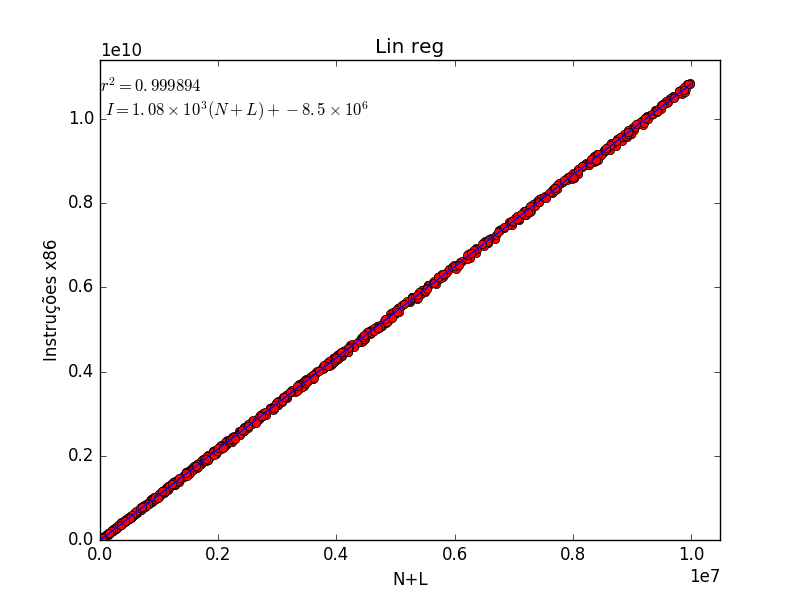
\includegraphics[width=0.5\textwidth]{../images/analiseExp_1e5.png}
	\caption{Análise experimental com parâmetros $2 \le N \le 10000 $ (1000 pontos)}
	\label{fig:analexp}
\end{wrapfigure}
Para se realizar a análise experimental temporal do algoritmo, foi utilizada a aproximação que cada instrução de C corresponde em média a um número fixo de instruções de CPU. Assim, em primeiro lugar procedeu-se à geração de $K$ diferentes casos de teste aleatórios (para cada caso foi escolhido aleatóriamente um $N$ e um $L\ge N-1$ e depois gerado um grafo conexo aleatório para esses parâmetros). De seguida, para cada caso de teste foi utilizada a ferramenta perf para contar o número de instruções de CPU utilizadas em modo utilizador durante a execução do program - $I$. Por fim, fez-se o plot do gráfico de $I$ em função de $N+L$. Obteve-se assim os resultados da Figura \ref{fig:analexp}.\par
Sendo o quoficiente de correlação linear muito próximo de 1 para todos os exemplos, a análise experimental comprova o resultado teórico esperado. \par
Encontra-se também em anexo testes executados mantendo a densidade do grafo aproximadamente constante, mas variando N [anexo A].
\section*{Análise assintótica espacial}
Como se verifica pelas estruturas utilizadas, o algoritmo utiliza 3 estruturas com $N$ inteiros (disco, low, parent), 1 estrutura com $N$ booleanos (AP), e uma estrutura com $N$ vetores, mas com no total $L$ inteiros no interior. Durante a recursividade, nunca é atingido um nível de profundidade superior a $N$, pelo que a memória de stack tem complexidade de pior caso $O(N)$ (num grafo linear). Assim a complexidade espacial será $O(N+L)$. Se não for contabilizada a memória utilizada para representar o grafo, o algoritmo tem complexidade espacial $O(N)$.

\section*{Prova de otimalidade do algoritmo}
Fácilmente se verifica que o algoritmo é ótimo com base no lema "o algoritmo ótimo para verificar se um nó é nó de corte tem complexidade de pior caso $\Omega(N+L)$".
Se para encontrar num grafo todos os nós de corte se tivesse complexidade assintóticamente inferior a $O(N+L)$, então seria possível utilizar esse algoritmo para verificar se um nó é nó de corte em tempo de pior caso inferior a $O(N+L)$, o que contradiz o lema, logo a complexidade estará em $\Omega (N+L)$. Pela nossa prova de correção e análise assintótica, o algoritmo de Tarjan corre em pior caso em $O(N+L)$, sendo portanto uma solução ótima $_\blacksquare$

Uma demonstração do lema baseia-se em não ser possível verificar para um grafo geral que $u$ é um nó de corte sem de facto percorrer todos os nós e arestas pelo menos uma vez, o que implica a complexidade de pior caso de  $\Omega (N+L)$.

\bibliography{ref}

\section*{ANEXO A - Análise experimental para $\sigma$ fixo}
\begin{figure}[H]
\subfloat[Análise experimental com parâmetros $202 \le N \le 1000 $ (1000 pontos) e $\sigma = 1\%$]{
	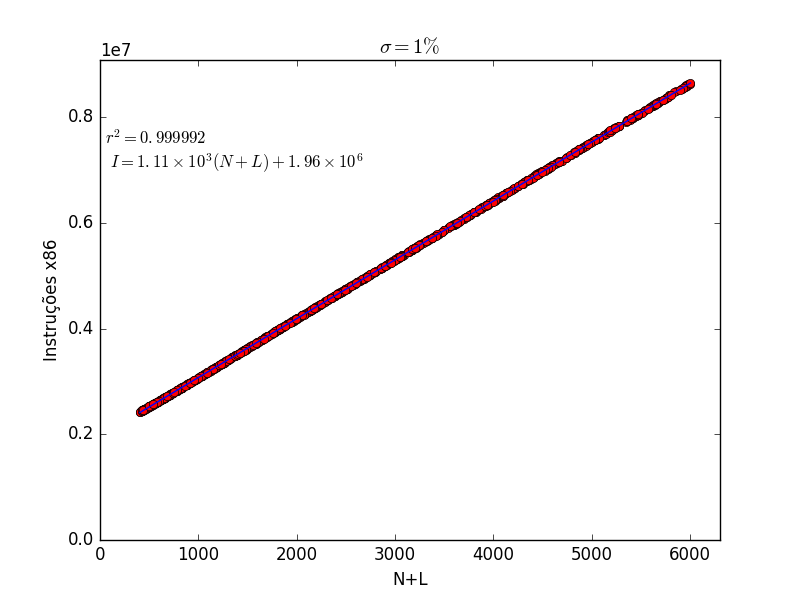
\includegraphics[width=0.45\linewidth]{../images/analiseExp_s1.png}
	\label{fig:analexp1}
}
\hfill
\subfloat[Análise experimental com parâmetros $22 \le N \le 1000 $ (1000 pontos) e $\sigma = 10\%$]{
	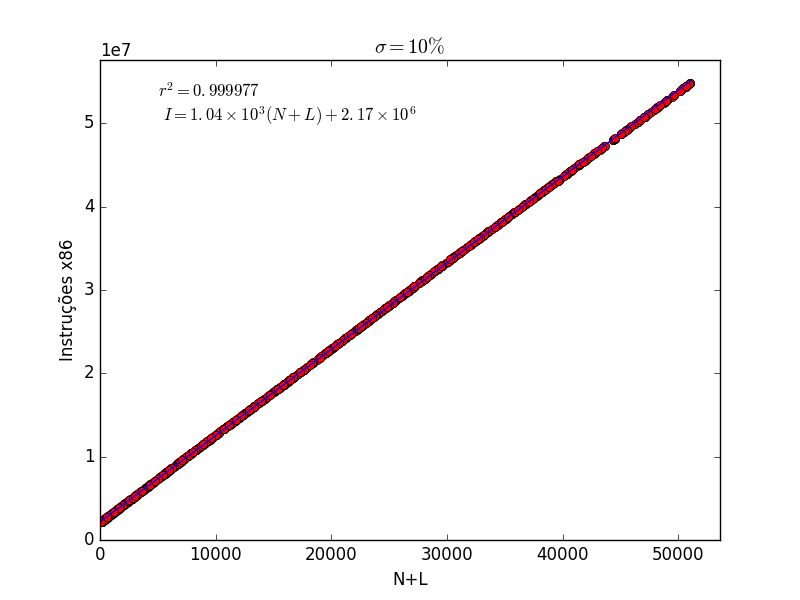
\includegraphics[width=0.45\linewidth]{../images/analiseExp_s10.png}
	\label{fig:analexp2}
}
\end{figure}
\begin{figure}[H]
	\subfloat[Análise experimental com parâmetros $6 \le N \le 1000 $ (1000 pontos) e $\sigma = 50\%$]{
		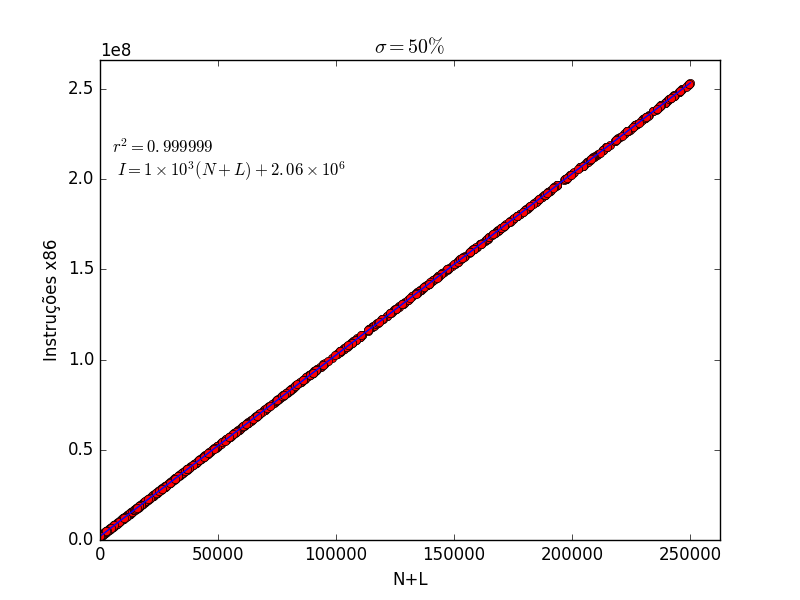
\includegraphics[width=0.45\linewidth]{../images/analiseExp_s50.png}
		\label{fig:analexp1}
	}
	\hfill
	\subfloat[Análise experimental com parâmetros $4 \le N \le 1000 $ (1000 pontos) e $\sigma = 100\%$]{
		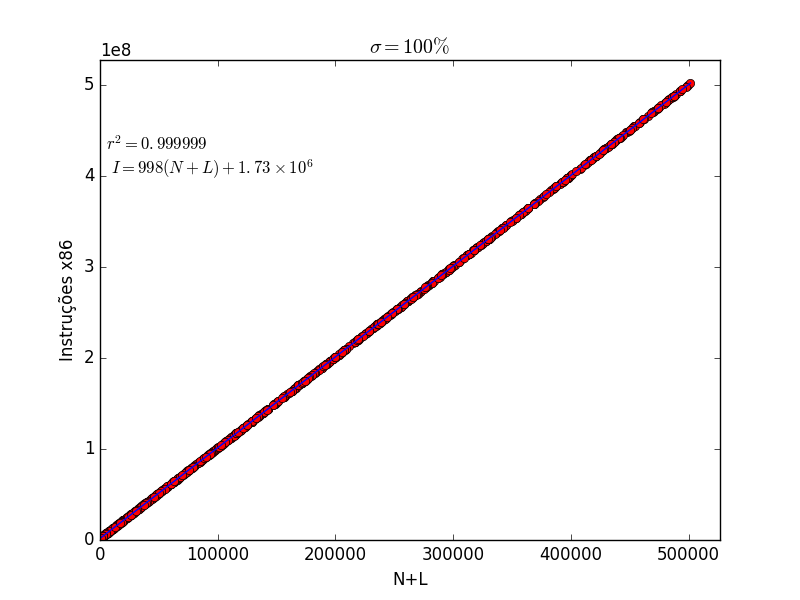
\includegraphics[width=0.45\linewidth]{../images/analiseExp_s100.png}
		\label{fig:analexp2}
	}
\end{figure}
\end{document}
